\documentclass[14pt]{extarticle}
\usepackage{amsmath}
\usepackage{amssymb}
\usepackage{gvv}
\usepackage{bm}
\usepackage{graphicx}
\title{\textbf{5.2.8}}
\author{\textbf{Aditya Mishra-EE25BTECH11005}}
\date{October 2, 2025}

\begin{document}
\maketitle

\section*{Question}
Solve the equations:
\begin{align*}
    5x - 3y = 11 \\
    -10x + 6y = -22
\end{align*}


\section*{Solution}
Forming the augmented matrix,
\[
\left(
\begin{array}{cc|c}
5 & -3 & 11 \\
-10 & 6 & -22 \\
\end{array}
\right)
\]

Perform row operations to reduce to row echelon form:

\[
\left(
\begin{array}{cc|c}
5 & -3 & 11 \\
-10 & 6 & -22 \\
\end{array}
\right)
\xrightarrow{R_2 \rightarrow R_2 + 2R_1}
\left(
\begin{array}{cc|c}
5 & -3 & 11 \\
0 & 0 & 0 \\
\end{array}
\right)
\]
The second row turns out to be all zeros, meaning the system is \\
dependent and consistent.

From the first row:
\[
5x - 3y = 11 \implies x = \frac{11 + 3y}{5}
\]

Let \(\vec{y} = \lambda, \lambda \in \mathbb{R}\) \\
Then, the general solution is:
\[
\boxed{
\vec{x} = \myvec{\frac{11}{5} \\ 0} + \lambda \myvec{\frac{3}{5} \\ 1}, \quad \lambda \in \mathbb{R}
}
\]
{\Large \textbf{Plot}}
\begin{figure}[!h]\centering
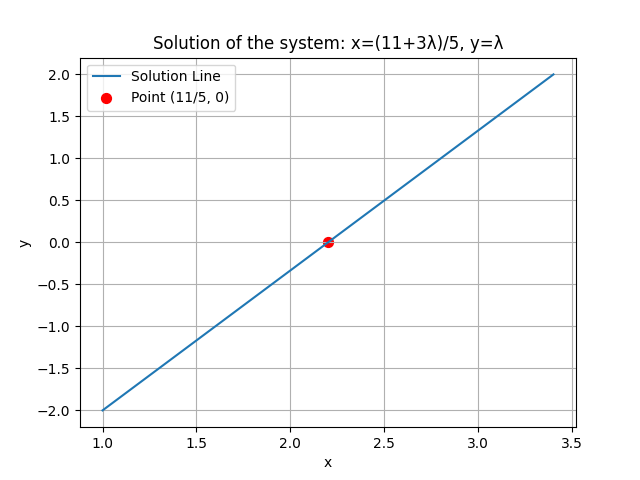
\includegraphics[width=0.9\columnwidth]{Figs/Figure_1.png}
\caption{2D plot of the solution}
\label{fig:plt}
\end{figure}
\end{document}

